\chapter{Sběr a analýza dat}
\label{chapter:data}
    Celý výzkum je možné rozčlenit do pěti fází/kroků, z nichž některé jsou zautomatizované a jiné je nutné realizovat manuálně. Ke sběru a analýze dat byly použity nástroj CrowdTangle, která je více popsán v sekci~\ref{sec:nastroje-analyzy} Nástroje analýzy a zdroje dat.
    
    V této kapitole je rozepsán průběh celého výzkumu od výběru vstupních stránek, přes sběr potřebných dat až po závěrečnou analýzu dat. 

\section{Doporučení a výběr vstupních stránek}
\label{sec:vyber-vstup-stranek}
    Před začátkem analýzy byla důležitá snaha pochopit, jak doporučené stránky funguji a jak se zobrazují. Proto byl v počáteční fázi výzkumu proveden krátký pretest, který se zaměřoval na to, zda je vůbec možné sbírat data o doporučova\-ných stránkách, jakým způsobem a zda bude lepší pracovat s anglickými nebo českými stránkami. Tento pretest byl nezbytný i proto, že se v průběhu práce na tomto výzkumu změnilo prostředí Facebooku, a tedy i možnosti sběru dat. V úplných počátcích bylo ještě možné doporučené stránky filtrovat pomocí url adresy, jak je zmíněno v úvodu předchozí kapitoly~\ref{chapter:design-vyzkumu}, což se nakonec ukázalo jako nefunkční způsob. 
    
    Během pretestu se mimo jiné ukázalo, že aktualizace se odrazily také na způsobu, jakým se zobrazují doporučované stránky. To znamená, že doporučení již nejsou na stránce automaticky viditelná. Aby se zobrazil seznam doporučených stránek, je nejdříve potřeba dát like stránce, pro kterou chceme doporučení zobrazit, a až poté se rozbalí výběr doporučení ve vrchní části (viz Obrázek~\ref{fig:fb-likedoporucenestranky}). Tento seznam je zobrazen do té doby, než dojde k aktualizaci stránky nebo přesunu na jiné místo na Facebooku. Pokud chceme znovu zobrazit doporučené stránky, je potřeba na stránce like zrušit a následně ho znovu obnovit. Doporučené stránky jsou tedy zobrazovány pouze omezeně za dodržení určitých postupů.
    
    Stránky nejsou ukázány všechny najednou, ale ve skupinách po čtyřech (viz Obrázek~\ref{fig:fb-likedoporucenestranky}). Pro zobrazení dalších je vždy potřeba posunout se ve výběru šipkou doprava. Celkově je těchto doporučených stránek 19. Je sice možné kliknout na tlačítko, které slibuje zobrazení více doporučení, ale v tomto seznamu jsou všechny různé stránky bez ohledu na vztah k předešlé stránce. 
  
    \begin{figure}[H]
        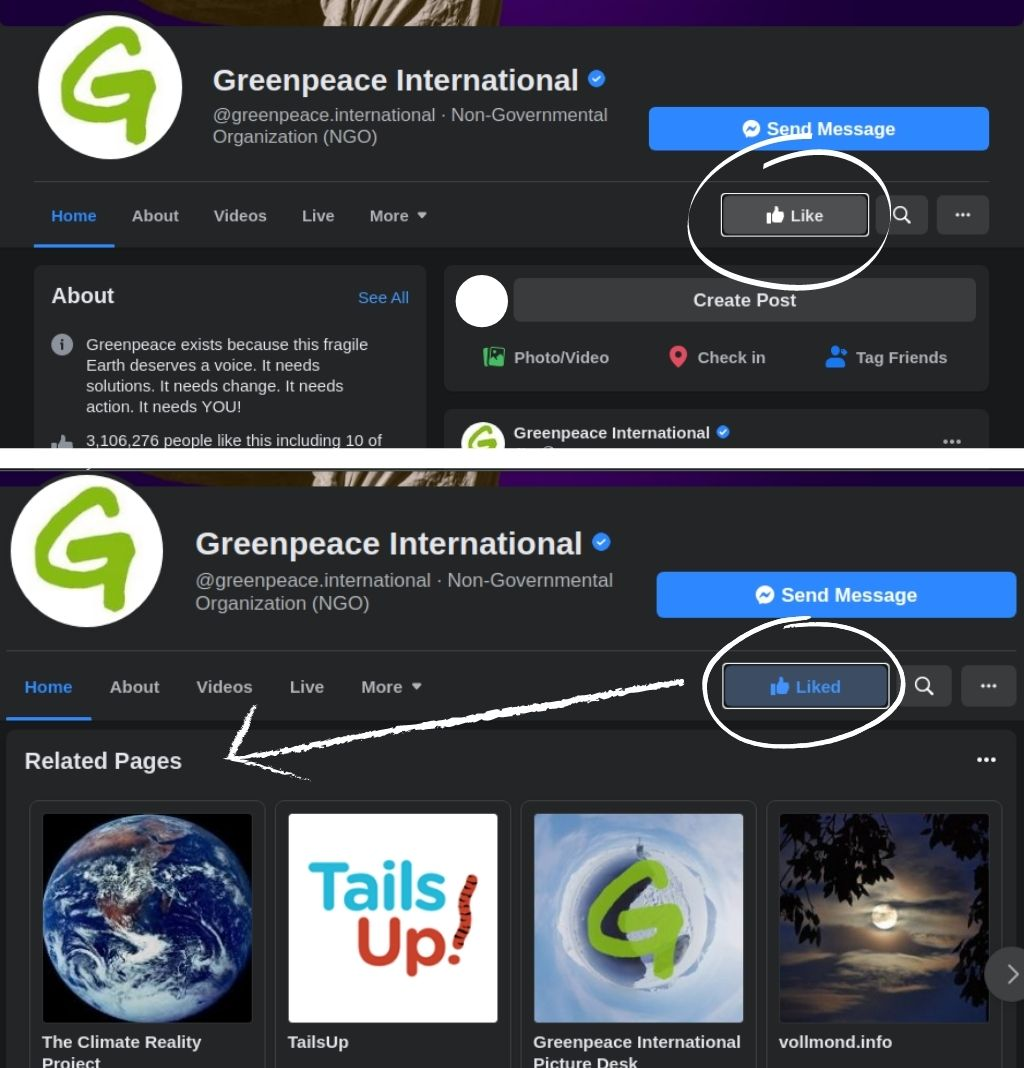
\includegraphics[width=\linewidth]{obrazky/like_doporucena (1).jpg}
        \centering
        \caption[Zobrazení doporučovaných stránek]{Zobrazení doporučovaných stránek. Zdroj: vlastní zpracování}
        \label{fig:fb-likedoporucenestranky}
    \end{figure}
  
    Není zcela jasné, podle jakého pravidla jsou stránky doporučovány. 19. března byl proveden test, kdy čtyři dobrovolníci propůjčili své profily a po zalikování totožných stránek se většině zobrazovaly prakticky totožné stránky jen s malými obměnami. O více než 20 dní později při testu na dalších třech osobách bylo v seznamu zobrazeno 11 odlišných stránek od těch z předchozího testu. Tito tři lidé však měli výčet doporučení na svých profilech také téměř totožný. Oba vzniklé seznamy doporučených stránek se prolínají. Nacházejí se v nich stránky, které mají podle tohoto pretestu silnou doporučovací hodnotu, neboť byly doporučeny všem zúčastněným, kteří poskytli náhled skrze své profily. Jsou to zejména ověřené stránky renomovaných organizací jako je Greenpeace, World Wild Fund, The Nature conservancy atd.  
    
    Výběr vstupních stránek probíhal manuálně dle kritérií stanovených v sekci \ref{sec:kategorizace-dat} Kategorizace dat. Předvýběr byl proveden už v rámci pretestu a následně byly vybrány pouze ty stránky, které nejvíce odpovídaly předurčeným požadavkům. Skrze funkci vyhledávání byla za pomoci klíčových slov cíleně provedena rešerše stránek \uv{pro} i \uv{proti} klimatické krizi. Vybrány byly první zobrazené výsledky odpovídající požadavkům - k tomu bylo potřeba stránku zobrazit a pečlivě prozkoumat její popis i obsah příspěvků. 
    
    Pokud tímto způsobem nebylo dohledáno odpovídající množství stránek, bylo použito právě rozšíření CrowdTangle pro prohlížeče, které umožňuje zjistit, jaké další stránky sdílely vybraný článek. Předpokladem je, že pokud například strán\-ka \uv{proti} sdílí protiklimatický článek, nabalí se další stránky s podobným postojem, které jej budou také sdílet. V krajním případě byly stránky vyhledávány skrze doporučení. Pokud již byla identifikovaná stránka \uv{proti}, skrze její doporučení byly vyhledány další podobné stránky. Vyhledávání stránek přes CrowdTangle a doporučení skrze již identifikované stránky bylo důležité především pro stránky \uv{proti}, které nebylo snadné dohledat přes facebookové vyhledávání.  
    
    Původně mělo být vybráno 10 stránek s pozitivním postojem a 10 stránek s negativním postojem ke klimatické krizi, ale během první fáze sběru dat se ukázalo, že jedna ze stránek \uv{proti} již zanikla a z toho důvodu již nebylo možné dále sbírat data. Proto byla náhodně odebrána jedna stránka z kategorie \uv{pro}. Z toho důvodu bylo nakonec vstupních stránek celkem 18. I při snížení počátečního vzorku stránek bylo stále možné získat dostatečné množství dat. 

    \setlength{\arrayrulewidth}{0.5mm}
    \setlength{\tabcolsep}{18pt}
    \renewcommand{\arraystretch}{2} 
     
    \begin{table}[h!] 
    \begin{center}
    \begin{tabular}{ | m{6cm}| m{5cm} | } 
    \hline
    \multicolumn{2}{|c|}{\Large \textbf{SEZNAM VSTUPNÍCH STRÁNEK}} \\
    \hline
    \textbf{stránky \uv{proti}} & \textbf{stránky \uv{pro}}  \\ 
    \hline
    CFACT & Greenpeace International \\ 
    \hline
    I Love Carbon Dioxide & NASA Climate Change \\ 
    \hline
    Climate Change LIES & Alliance for Climate Education \\ 
    \hline
    Australian Climate Madness & Climate Change Is Real \\ 
    \hline
    Climate Depot & Climate Reality \\ 
    \hline
    Climate Change Dispatch & Climate Change News \\ 
    \hline
    CO2 Coalition & Nature Climate Change \\ 
    \hline
    Global Warming, Climate Change, whatever it's called, is a scam. & Stop Global Warming \\ 
    \hline
    Global Climate Scam & Global Warming \\ 
    \hline
    \end{tabular}
    \caption{Seznam vstupních stránek}
    \label{table:seznam-vstupnich-stranek}
    \end{center}
    \end{table}
    
\section{Sběr stránek první a druhé úrovně}
\label{sec:sber-prvni-druha-uroven}
    Primární stránky jsou výchozím bodem pro další sběr dat. Jestliže každá (vstupní) stránka doporučuje až 19 dalších podobných stránek, to znamená při dvoustupňovém sběru dat tisíce stránek - přesněji až $19^2$. Zaznamenávat takové množství stránek manuálně by bylo přinejmenším časově náročné. Proto byla tato část (stejně jako některé další části) realizována strojově. 
    
    Strojový sběr dat byl uskutečněn za použití „scriptu“ v programovacím jazyce Python realizovaný s použitím knihovny Selenium, které umožňuje zautomatizování jednotlivých příkazů v interakci s prohlížečem.~\citep{pypi}. 
    
    Zjednodušeně proces vypadal asi takto: S pomocí knihovny Selenium se automaticky otevře prohlížeč a načte se jedna z vybraných vstupních Facebookových stránek. Aby bylo možné dát stránce like a zobrazit tak seznam doporučených stránek, je potřeba se přihlásit. Program se proto přihlásí k soukromému facebookovému účtu za pomocí osobních přístupových údajů (e-mail a heslo). Po zobrazení seznamu doporučených stránek je pro každou z nich stažen její název a url adresa. Nakonec je na každé stránce zrušeno likování. 
    
    Tento postup byl následně aplikován na každou další vstupní nebo sekundární stránku. Stahovány tedy byly doporučené stránky ze vstupních stránek - tzn. sekun\-dární stránky (18 stránek a na každé z nich 19 doporučených je 342) - a následně stránky doporučené na sekundárních stránkách - tedy terciární (342 stránek a na každé z nich 19 doporučených je 6 498 stránek). U těchto stránek druhé úrovně už dále nebyly zaznamenávány další doporučení. 
    
    Sběr všech dat nemohl proběhnout zároveň a najednou, ale musel být uskuteč\-něn ve třech fázích s jistými časovými rozestupy. Nedlouho po spuštění programu totiž narazil tento zautomatizovaný proces na bariéru Facebooku, která je vystavěna proti robotům a nevyžádaným strojovým akcím. Jinými slovy systém Facebooku rozpoznal, že aktivitu na stránkách neprovádí člověk, ale jiný algoritmus. Kromě varování ještě Facebook jako sankci za toto chování na několik dní zablokoval na účtu, který byl používán k přihlášení, možnost stránky likovat. Tato restrikce, ale byla za několik dní uvolněna a následně byl sběr dat preventivně rozložen do kratších úseků. 
    
    Aby mohly být všechny stránky později filtrovány a mohly být vybrány jen ty, které jsou pro výzkum relevantní, byl uskutečněn dodatečný sběr dat facebookových příspěvků. Pro všechny stránky v nově vytvořeném datasetu bylo za pomocí knihovny fb-scraper\footnote{https://github.com/kevinzg/facebook-scraper}, která umožňuje stahovat informace o veřejných stránkách bez API klíče, staženo přibližně třicet až čtyřicet příspěvků z jejich vlastního facebookového feedu, s cílem využít je v další fázi výzkumu~\citep{pypi_2021}. 
    
    \begin{figure}[H]
        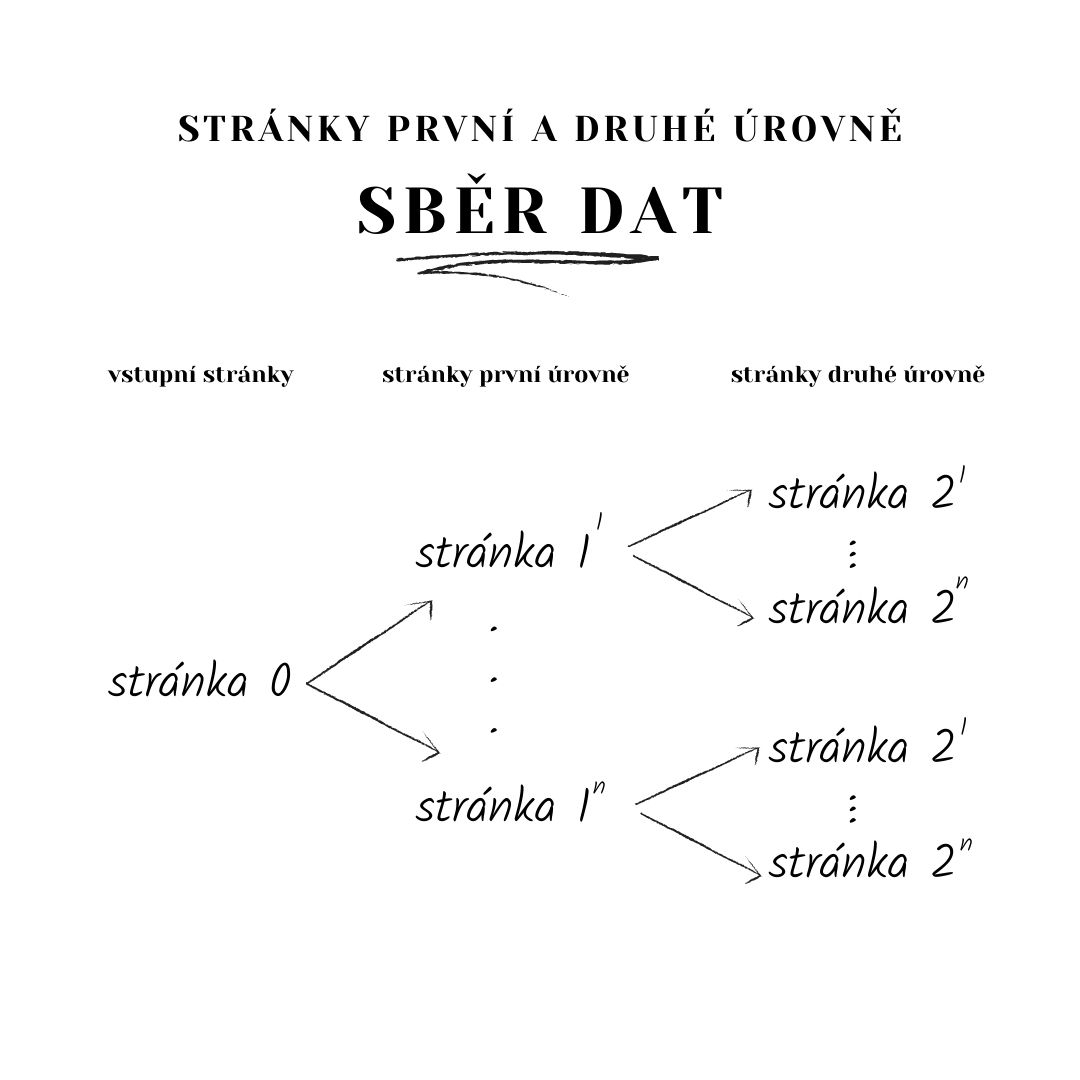
\includegraphics[width=\linewidth]{obrazky/sber_dat.jpg}
        \centering
        \caption[Schéma víceúrovňového sběru dat]{Schéma víceúrovňového sběru dat. Zdroj: vlastní zpracování}
        \label{fig:fb-sber-dat}
    \end{figure}
  
\section{Klasifikace stránek}
\label{sec:cisteni-klasifikace-dat}
    V doporučených stránkách se nemusí vždy nutně vyskytovat pouze stránky o klimatické krizi, ale mohou zde být i další podobné stránky (například takové, které spadají do stejné předdefinované kategorie facebookových stránek jako jsou třeba neziskové organizace nebo veřejně známá osobnost), proto byly vyfiltrovány a vyřazeny ty stránky, které se klimatickou krizí nezabývají. Tento krok je mimo jiné důležitý také pro následující fázi, ve které se stahuje mnohem větší množství příspěvků. Tímto včasným filtrováním se uspoří čas a prostor na pevném disku. Nakonec bylo nutné každou stránku klasifikovat jako \uv{pro} nebo \uv{proti} klimatické krizi. 
    
    Původně bylo zamýšleno, že ke kategorizaci dat v této fázi bude použit nástroj LIWIC\footnote{Zkrácený název pro Linguistic Inquiry and Word Count}, který slouží k analýze emocionálních, kognitivních a strukturálních komponentů nejen psaného textu. To se nakonec při bližším prozkoumání této metody ukázalo jako nevhodné a neúčinné.~\citep{pennebaker2015development} Místo toho byly použity jiné metody. Část tohoto procesu byla uskutečněna strojově a část manuálně se záměrem dosáhnout co nejpřesnějších výsledků. 
    
    Nejdříve bylo potřeba určit, které stránky nejvíce odpovídají tématu klimatické změny/klimatické krize. K tomu posloužily příspěvky, které byly staženy v předchozí fázi výzkumu. Tento balík přibližně třiceti až čtyřiceti příspěvků získaný pro každou ze stránek z datasetu (vstupní, sekundární, terciární) sloužil jako podklad pro klasifikaci. Klasifikace byla provedena na základě vytvořeného skóre, které určovalo, do jaké míry se stránka zabývá klimatickou krizí. 
    
    Před samotným výpočtem skóre a klasifikací bylo potřeba jazyková data (pří\-spěvky) předzpracovat. Za tímto účelem byly příspěvky tokenizovány - rozsekány na jednotlivá slova a převedena na malá písmena. Aby bylo dosaženo větší úspěš\-nosti při strojové identifikaci jednotlivých slov, byla všechny slova v příspěvcích lematizována. To znamená, že byla převedena na slovníkové tvary. Tato úprava umožňuje postihnout i případy kdy je slovo relevantní, ale není obsaženo v našich klíčových slovech. Pro ilustraci slovo going bude převedeno na tvar go. Následně byly odstraněny takzvané „stopwords“ - slova, které mají vysokou četnost a při zpracování přirozeného jazyka nepřinášejí téměř žádnou informaci, a proto se z textu odstraňují. Jinými slovy se jedná nadbytečná slova jako „the“, „a“, „it“ atd.  
    
    Pro předem definovaná klíčová slova \emph{climate, warming, CO2 a change} bylo vypočítáno vlastní skóre - pozitivní číslo, které vyjadřuje relevantnost daného příspěvku. Čím vyšší měla daná stránka toto skóre, tím více odpovídala tématu klimatické krize. 
    
    Je potřeba dodat, že výše zmíněná slova byla vybrána realizátorkou výzkumu na základě jejích osobních preferencí. Přestože byla vybrána taková slova, která podle ní nejvíce charakterizovala dané téma, tento výběr můžeme být zatížen určitým zkreslením. V nejhorším případě mohly být z výběru diskvalifikovány některé stránky \uv{pro} nebo \uv{proti}, které na svých stránkách častěji používají jiná slova, přestože mluví o klimatické krizi. 
    
    Skóre pro jednotlivé stránky byla počítána vlastním způsobem, který je kombinací klasického modelu TF-IDF\footnote{Term Frequency-Inverse Document Frequency je metoda, která měří, relevanci mezi texty a je typicky používaná pro vyhledávání v dokumentech.~\citep{ullman2011mining}} a BM25\footnote{BM25 je metoda, která také vrací relevanci mezi texty, ale provádí komplexnější výpočet.~\citep{article}}, respektive jeho TF částí. Nejdříve byly všechny příspěv\-ky pro danou stránku sloučeny do jediného dokumentu - tento postup byl následně proveden pro všechny stránky. V každém takovém dokumentu (specifickém pro každou ze stránek) byl vypočítán celkový počet výskytů klíčových slov (term-frequency). Aby výsledné skóre reflektovalo rozdílnou délku dokumentů (Krátký dokument obsahující stejný počet klíčových slov jako dlouhý dokument bude mít vyšší skóre.), byla tato četnost klíčových slov vynásobena vážícím koeficientem, který byl spočítán jako medián délky všech dokumentů a vydělen délkou dokumentu (počtem slov) specifického pro stránku, pro kterou bylo skóre počítáno. 
    
    Nakonec byl výsledný seznam stránek první a druhé úrovně (tedy bez osmnácti vstupních stránek) manuálně zkontrolován a každé ze stránek byla přiřazena „nálepka“ podle jejího vztahu ke klimatické krizi - to znamená \uv{proti} nebo \uv{pro}. Část stránek byla vyřazena pokud i přes tento postup neodpovídala definici stránek, které se zabývá klimatickou krizí. Některé stránky byly nakonec odstraněny neboť z nějakého důvodu již nebyly funkční či relevantní. Například stránku IISDRS není možné načíst a stránka REDD+ Ethiopia byla napadena hackery. 
  
\section{Stažení podrobných dat o příspěvcích}
\label{sec:stazeni-dodatecnych-dat}
    V neposlední řadě byla stažena dodatečná data ke všem stránkám, které se zabývají klimatickou krizí - stránkám, které prošly klasifikací a filtrováním v předchozím kroku. Tyto dodatečná data mohou posloužit k analýze souvislostí mezi doporučováním určité stránky a jejím obsahem nebo počtem interakcí. Například zda si vedou v oblasti interakcí lépe stránky \uv{pro} nebo \uv{proti} klimatické krizi.
    
    Ke stažení dodatečných informací o příspěvcích na všech stránkách, které vzešly z fáze očištění a klasifikace dat, byl použit nástroj CrowdTangle, který umožňuje analyzovat sociální sítě.~\citep{crowdtangle_2021} Dodatečná data obsahují informace o přibližně třiceti tisících příspěvků včetně názvu, ID a uživatel\-ského jména stránky nebo počtu „followerů“ v době zveřejnění příspěvku atd. Konkrétní informace o příspěvcích zahrnují mimo jiné datum zveřejnění příspěvku, počet a druh interakcí, druh příspěvku (video, foto, link\dots), url odkazu.   
  
\section{Analýza dat}
\label{sec:analyza-dat}
    Poslední, a zároveň tou nejdůležitější částí tohoto výzkumu je vyhodnocení dat s ohledem na výzkumné otázky a stanovené cíle. Analýza je založena na informacích, které byly získány na základě postupu, který byl popsán výše v této kapitole. 
    
    Včetně vstupních stránek zůstalo v datasetu po vyčištění celkově 280 unikát\-ních stránek. Z nichž pouhých 40 bylo proti klimatické změně a zbylých 240 mělo k této tématice kladný postoj\footnote{Způsob zařazení stránek viz kapitola 7.3 Očištění a klasifikace dat nebo více o kategorizaci dat v kapitole 6.1 Kategorizace dat.} Žádná z osmnácti vstupních stránek nebyla dále doporučena mezi stránkami první ani druhé úrovně až na Stop Global Warming, která se následně objevila přesně jednou (celkově tedy dvakrát). 
    
    V doporučení se (včetně duplikací) objevilo 658 relevantních stránek. Z toho 540 bylo s pozitivním vztahem k existenci klimatické změny a 147 s negativním postojem k existenci klimatické změny. 
    
    \begin{figure}[ht]
        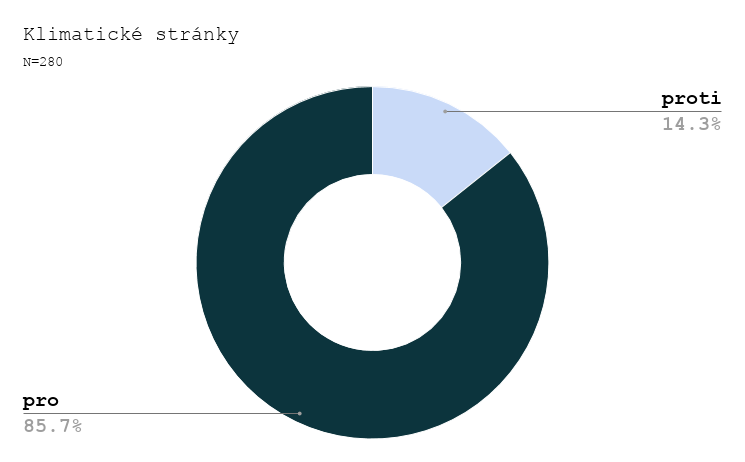
\includegraphics[width=11cm]{obrazky/Klimatické stránky N=280.png}
        \centering
        \caption[Poměr klimatických stránek podle kategorie]{Poměr klimatických stránek podle kategorie. Zdroj: vlastní zpracování}
        \label{fig:fb-klima-stranky-kategorie}
    \end{figure}

    Přestože je stránek \uv{proti} šestkrát méně než stránek \uv{pro}, v celkovém datasetu doporučených stránek se častěji opakují oproti stránkám \uv{pro}. Což může být právě tím, že těchto stránek není tolik, a proto má Facebook menší výběr stránek, ze kterých může pro doporučování čerpat. Zatímco stránky \uv{pro} se objevují v doporučení průměrně přibližně dvakrát, stránky \uv{proti} více než třikrát. Zatímco v první úrovni je doporučeno 21 unikátních stránek \uv{proti} v další úrovni už je to jen 10 unikátních stránek. Doporučení negativních stránek je tedy prakticky vyčerpáno už mezi vstupními daty a daty první úrovně.  

    \begin{figure}[H] 
        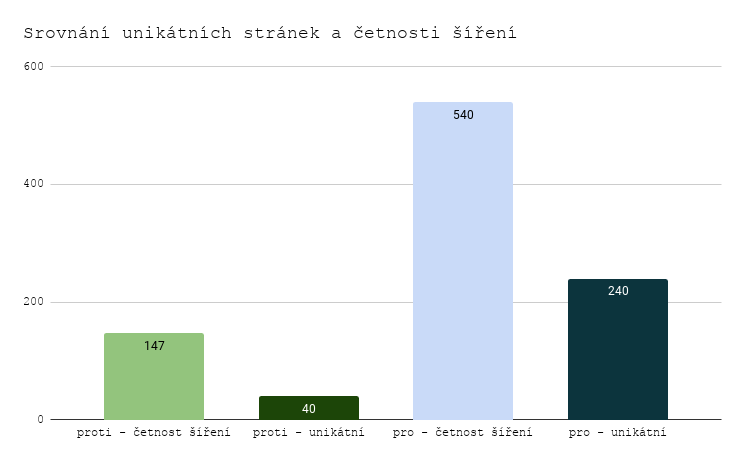
\includegraphics[width=14cm]{obrazky/Srovnání unikátních stránek a četnosti šíření.png}
        \centering
        \caption[Srovnání unikátních stránek vzhledem k četnosti šíření]{Srovnání unikátních stránek vzhledem k četnosti šíření. Zdroj: vlastní zpracování}
        \label{fig:fb-klima-stranky-sireni}
    \end{figure}

    Konkrétně je v celém datasetu stránka s pozitivním postojem k existenci klimatické změny průměrně doporučována 2,25x s medianem 1 a stránka s negativním postojem ke klimatické změně 3,68x se střední hodnotou 3. S tím, že nejčastěji je u obou kategorií stránka doporučena pouze jednou. 
    
    Méně než polovina všech stránek (bez ohledu na postoj ke klimatické změně), přesněji 134, byla doporučena více než jednou. Pouze 25 stránek mělo více než 5 doporučení a jen 8 stránek mělo 10 a více. Konkrétní seznam stránek těchto osmi stránek je možné si prohlédnou v tabulce~\ref{table:nejcasteji-sirene-stranky} Nejčastěji šířené stránky. 
    
    Jedná se o stránky jak velkých mezinárodních organizací jako je Greenpeace nebo Organizace spojených národů, tak o menší stránky se středním i nižším počtem followerů. Na první pohled vyčnívá stránka Lord~Monckton, která má vzhledem k ostatním stránkám jen okolo 9,5 tisíc sledujících a zároveň ve svém názvu nijak nenaznačuje spojitost s klimatickou změnou - ovšem při bližším prozkoumání stránky a jejích příspěvků je vidět, že toto téma je často zmiňováno jak v příspěvcích, tak v samotném popisu stránky, kde je Lord~Monckton označován jako odborník na klimatickou změnu. Jako svou webovou stránku taktéž uvádí web CFACT, který může být považován za proti klimatický portál. Další stránkou, která se výrazně vyčnívá je Above~Climate~Change s pouhými 367 followery. 
    
    Přestože jsou stránky s negativním postojem ke klimatické změně doporučová\-ny více (z pohledu frekvence doporučování) než stránky pro klimatickou změnu, mezi výběr osmi nejšířenějších stránek se dostalo více \uv{pro} nežli \uv{proti}. Konkrétně je rozložení stránek v poměru 5:3. Vysvětlení může být více: ať už celkově výší počet followerů u stránek \uv{pro} nebo lepší publicita a větší kredibilita stránek velkých organizací jako je Greenpeace nebo OSN.

    \setlength{\arrayrulewidth}{0.5mm}
    \setlength{\tabcolsep}{25pt}
    \renewcommand{\arraystretch}{2} 
    
    \begin{table} [h!] 
    \centering
    \resizebox{\textwidth}{!}{
    \begin{tabular}{| m{4cm}| m{1.7cm} | m{1.2cm} | m{1.7cm} |} 
    \hline
    \multicolumn{4}{|c|}{\Large \textbf{8 NEJŠÍŘENĚJŠÍCH STRÁNEK}}   \\ 
    \hline
     \textbf{Název stránky} & \textbf{Vztah ke klimatické krizi} & \multicolumn{1}{c|}{\textbf{Doporučení}} & \multicolumn{1}{c|}{\textbf{Followers}}            \\ 
    \hline
    Lord Christopher Monckton, 3rd Viscount Monckton of Brenchley & proti & 17 & 9 444 \\ 
    \hline
    Friends of Science & proti & 14 & 34 198 \\ 
    \hline
    Skeptical Science & pro & 13 & 183 498 \\ 
    \hline
    Inside Climate News & pro & 13 & 81 086 \\ 
    \hline
    Climate Home News & pro & 12 & 18 810 \\ 
    \hline
    Above~Climate~Change & proti & 10 & 367 \\ 
    \hline
    Greenpeace USA & pro & 10 & 726 174 \\ 
    \hline
    UN Environment Programme & pro & 10 & 1~094~527 \\
    \hline
    \end{tabular}
    }
    \caption{Nejčastěji šířené stránky}
    \label{table:nejcasteji-sirene-stranky}
    \end{table}

\subsection{Prolomení bubliny}
\label{sec:prolomeni-bubliny}
    K pochopení, jakým způsobem je analyzováno prolomení filtrační bubliny, je důležité porozumět tomu, že prolomení může být identifikováno pouze existuje-li spojení mezi výchozí stránkou a dalšími stránkami, které doporučuje. Těmito výchozími stránkami mohou být v tomto případě pouze stránky vstupní a první úrovně. Těchto stránek, nepočítáme-li jejich duplikace, je v kategorii \uv{pro} 67 a v \uv{proti} 20. Zbylé stránky jsou stránky druhé úrovně u kterých už nejsou v rámci tohoto výzkumu uvažovány/promítnuty žádné další doporučení. Proto mají stránky druhé úrovně spíše referenční funkci ke stránkám první úrovně. 
    
    Při prozkoumání „větve“ doporučení, která vychází ze vstupních stránek akceptujících existenci klimatické krize, se ukazuje, že jsou zde doporučovány téměř výhradně stránky se stejným postojem. V celém řetězci (mezi první a druhou úrovní) se objevuje jen 7 stránek \uv{proti} klimatické změně a na druhou stranu je zde doporučeno 429 stránek se stejným postojem jako mají vstupní stránky. Na každou stránku bylo průměrně doporučeno přibližně 6.5 relevantních stránek. Z toho průměrně 6.3 bylo \uv{pro} a jen 0.1 \uv{proti}, což vypovídá o téměř nulovém prolomení filtrační bubliny. 
    
    Stránky, které souhlasí s existencí klimatické změny a byla u nich prolomena filtrační bublina, jsou v porovnání k některým ostatním stránkám \uv{pro} vzhledem k počtu fanoušků spíše střední, až menší velikosti. Nejedná se o stránky se statisící fanoušky a jsou zde stránky, které mají jen několik tisíc followerů. Stránka s největším počtem fanoušků má 60 600 a stránka s nejmenším počtem jen 2 280.
    
     \setlength{\arrayrulewidth}{0.1mm}
    \setlength{\tabcolsep}{40pt}
    \renewcommand{\arraystretch}{1}
    \begin{table}[h!] 
        \centering
        % \resizebox{\textwidth}{!}{%
        \begin{tabular}{| m{2cm} | m{1.7cm} | m{2cm} |} 
            \hline
            \multicolumn{3}{|c|}{\Large \textbf{Prolomení bublin stránky \uv{pro} }} \\ 
            \hline
            \textbf{Název stránky} & \textbf{Počet prolomení} & \textbf{Followers} \\ 
            \hline
            Citizens Climate Lobby  & 1 & 41 471 \\ 
            \hline
            I Heart Climate Scientists  & 1 & 60 601 \\ 
            \hline
            Global Warming Fact of the Day  & 1 & 10 927 \\ 
            \hline
            Our Children's Trust  & 1 & 29 640 \\ 
            \hline
            Global Warming Climate Change Report  & 1 & 13 524 \\ 
            \hline
            Climate Change is Real  & 1 & 2 280 \\ 
            \hline 
            Mothers for Nuclear  & 1 & 6 590 \\ 
            \hline
        \end{tabular}%
        % }
        \caption{Stránky \uv{pro}, v jejichž doporučení byla prolomena bublina.}
        \label{table:prolomeni-bubliny-pro}
    \end{table}
    
    Stránky \uv{proti}, které prolomily filtrační bublinu stránek s pozitivním postojem k existenci klimatické změny byly pouze čtyři - Climate Change Facts, Refutations to Anti-Nuclear Memes, The Global Warming Policy Forum, Dr. James E. Hansen. - z nichž 3 prolomily každá jednu stránku \uv{pro} a jedna ze stránek opakovaně prolomila více stránek. Jednalo se o stránku Dr. James E. Hansen. 
    
    Při sledování vývoje doporučení vycházejícího ze vstupních stránek, které popírají existenci klimatické krize, jsou výsledky příznivější ve prospěch prolamování filtračních bublin. Relevantních stránek je v tomto případě méně, průměr\-ně 4.8, a připadá na ně zhruba 3.4 proti klimatických stránek. Což je sice pořád hodně, ale na druhou stranu každá stránka (vstupní nebo první úrovně) doporučuje v průměru 1.5 stránky s opačným postojem ke klimatické krizi. Takže z každého doporučení je teoreticky možné dostat se alespoň na jednu stránku s opačným názorem na toto téma. V praxi ale některé stránky \uv{proti} doporučují více stránek \uv{pro} a z toho důvodu jen u patnácti stránek \uv{proti} dojde k prolomení filtrační bubliny.
    
    Stránky, které nesouhlasí s existencí klimatické změny mají obecně méně fanoušků než stránky s opačným postojem. Vzhledem k tomu, že nad otázkami klimatické změny panuje vědecký konsensus, je logické, že odpůrců tohoto postoje je menšina. Narozdíl od stránek \uv{proti} se mezi stránkami \uv{pro}, jak už bylo řečeno, nachází i stránky velkých známých mezinárodních organizací, které mají statisíce fallowerů. V kontrastu jedna z největších stránek, která jde proti klimatu s názvem CFACT, má jen 61 157 followerů. Proto i v tabulce prolomení filtračních bublin stránek \uv{proti} jsou spíše stránky menší velikosti. Rozpětí je však velmi široké od 464 fanoušků až po 34 188. Dvě nejmenší stránky také dostaly dvě nejvyšší prolomení. 
    
    \setlength{\arrayrulewidth}{0.5mm}
    \setlength{\tabcolsep}{60pt}
    \renewcommand{\arraystretch}{1.5} 
    
    \begin{table} [ht] 
    \centering
    \resizebox{\textwidth}{!}{%
    \begin{tabular}{| m{4cm}| m{1.5cm} | m{2cm} |} 
    \hline
    \multicolumn{3}{|c|}{\Large \textbf{Prolomení bublin stránky \uv{proti} }}   \\ 
    \hline
    \textbf{Název stránky} & \textbf{Počet prolomení} & \textbf{Followers}            \\ 
    \hline
    Climate Change Facts  & 10 & 464 \\ 
    \hline
    The Global Warming Policy Forum & 5 & 14 124 \\ 
    \hline
    Climate Change and Global Warming - Exposed  & 5 & 528  \\ 
    \hline
    Is There Global Cooling  & 4 & 2 525 \\ 
    \hline
    Climate Change Dispatch  & 3 & 6 036  \\ 
    \hline
    Climate Change LIES  & 3 & 16 238  \\ 
    \hline
    Climate News  & 3 & 3 149 \\ 
    \hline
    I love Carbon Dioxide  & 2 & 19 847 \\ 
    \hline
    wattsupwiththat  & 2 & 13 017 \\ 
    \hline
    Global Climate Scam  & 2 & 1 254 \\ 
    \hline
    CO2 Coalition  & 1 & 6,056 \\ 
    \hline
    World Wide Protest Against the Global Warming SCAM  & 1 & 1 152 \\ 
    \hline
    Center for Industrial Progress  & 1 & 5 749 \\ 
    \hline
    Global Warming, Climate Change, whatever it's called, is a scam.  & 1 & 1 611 \\ 
    \hline
    Friends of Science  & 1 & 34 188 \\ 
    \hline
    \end{tabular}%
    }
    \caption{Stránky \uv{proti}, v jejichž doporučení byla prolomena bublina.}
    \label{table:prolomeni-bubliny-proti}
    \end{table}
    
    Mimo jiné je zajímavé, že se počty prolomení u stránek jeví bez na první pohled jasného vzorce. Stránka Climate Change Facts má 10 opačných doporučení, zatímco stránky Climate Change and Global Warming - Exposed a The Global Warming Policy Forum, které jsou v počtu prolomení na druhém místě, mají jen 5 názorově odlišných doporučení. Následně už doporučení klesají vždy o jedno číslo. Vysvětlení tohoto jevu by mohlo být v zásadě jednoduché. Některé stránky se v datasetu opakují, a tudíž mají teoreticky i větší šanci několikrát prolomit filtrační bublinu.
    
    Doporučení by se také mohly odvíjet od názvů stránek. Například stránka Climate Change Facts na první pohled vypadá jako stránka, které pravdivě informuje o klimatické změně. To by mohlo být jedno z vysvětlení pro skokový rozdíl v doporučení oproti ostatním stránkám.
    
    Jedná se však o pouhou domněnku, která pravděpodobně nebude jediným faktorem, který hraje v doporučení roli. Mezi stránkami, které bublinu prolomily, jsou totiž i takové, které už ve svém názvu vyjadřují jasný nesouhlasný postoj ke klimatické změně. Jsou to stránky Climate Change LIES; Global Climate Scam; World Wide Protest Against the Global Warming SCAM; Global Warming, Climate Change, whatever it's called, is a scam. Několik stránek pak svůj postoj vyjadřuje nepřímo, například zaobalením do ironie jako: Is There Global Cooling nebo I love Carbon Dioxide. Název by mohl být pro zařazení stránek významný - vyjádření postoje by mohlo třídění doporučení usnadnit a při použití ironie nebo věrohodného názvu by naopak mohla být stránka zařazena chybně. 

    
    Stránek, které prolomily filtrační bublinu na stránkách, které se vyhraňují proti existenci antropocentrické klimatické změny, bylo celkově třicet dva. Osmi z nich se podařilo bublinu prolomit u více než jedné stránky. Z nich u dvou byly prolomeny tří a u jedné čtyři stránky. Nejúspěšnější stránky v tomto prolamování byly v pořadí od nejvíce prolomení po nejméně tyto stránky: Skeptical Science, Climate Home News, Bulletin of the Atomic Scientists, Mothers for Nuclear, Climate Change In Pictures, Global Warming Planet, Global Warming Times, Climate Discussion Nexus.
    
    \begin{figure}[H]
        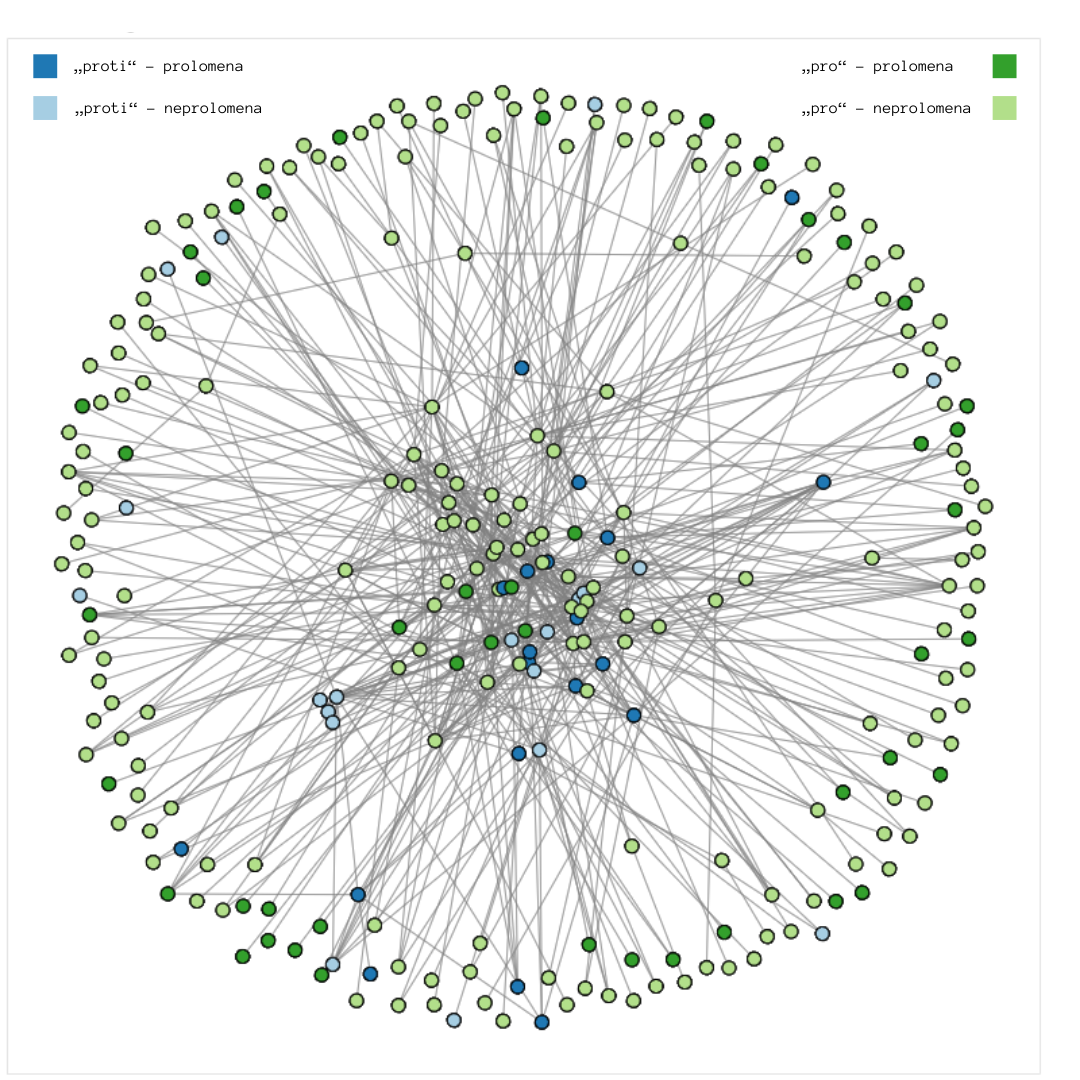
\includegraphics[width=13cm]{obrazky/prolomenibublinymapa_spopisky.png}
        \centering
        \caption[Mapa prolomení filtračních bublin]{Mapa prolomení filtračních bublin. Zdroj: Vlastní zpracování}
        \label{fig:fb-klima-stranky-bubliny}
    \end{figure}
    


%-------------------------------------------------------------------------------

\subsection{Interakce na stránkách a jejich příspěvky}
\label{sec:interakce}
    Pro lepší porozumění tomu, zda může mít na četnost šíření stránek a prolamování filtračních bublin vliv engagement, jak bylo naznačeno v sekci~\ref{sec:doporucovaci-algoritmus-engagement} Doporučovací algoritmus - za vším hledej engagement, byla také provedena analýza, která se zaměřovala na reakce na stránkách s pozitivním i negativním postojem ke klimatické změně. 
    
    Jak se ukazuje, stránky \uv{pro} mají v průměru asi jednou tolik interakcí na stránku, jako stránky \uv{proti}. Konkrétně je to 14 746 ku 6 968. U stránek \uv{pro} je průměrně 105 interakcí a u stránek s negativním postojem k existenci klimatické změny je to 67 na příspěvek. 
    
    V potaz však musí být brán i počet followerů na stránkách s pozitivním i negativním postojem k existenci klimatické krize. Stránky \uv{pro} mají v průměru téměř $36\times$ více fanoušků než stránky \uv{proti}. A zatímco na každého fanouška stránky \uv{pro} připadá průměrně 0.0012 reakcí, na každého fanouška stránky \uv{proti} je to 0.0065 reakcí. Lidé, kteří sledují stránky s negativním postojem k existenci klimatické změny, tedy s příspěvky interagují více. 
    
    %Při bližším pohledu na průměr jednotlivých reakcí\footnote{Angry, sad, shares, love, wow, care, comments, haha a likes.} stránky \uv{pro} nedosahují v žádném z případů ani poloviny průměrných hodnot stránek s pozitivní postojem k existenci klimatické změny. Nejvíce se stránky \uv{proti} blíží stránkám \uv{pro} v průměrných hodnotách interakcí v použití reakcí „haha“, sdílení a komentář. 
    
    %\begin{figure}[H]
        %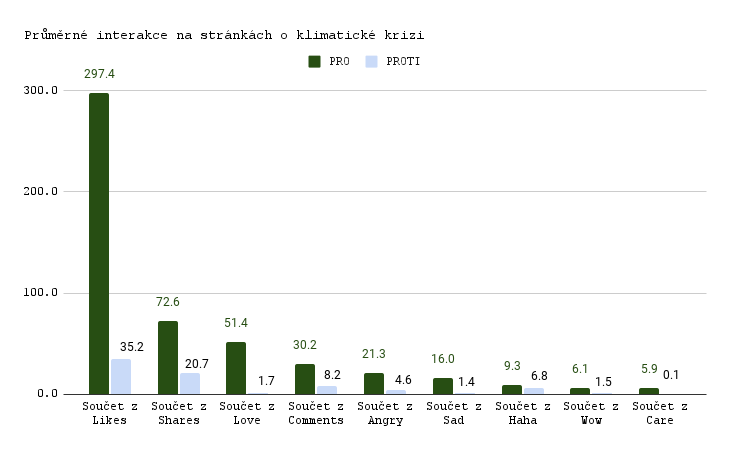
\includegraphics[width=14cm]{obrazky/Interakce na stránkách.png}
        %\centering
        %\label{fig:fb-klima-stranky-interakce}
        %\caption{Průměrné interakce na stránkách \uv{pro} i \uv{proti}. Zdroj: vlastní zpracování}
   % \end{figure}
    
    Při bližším pohledu na konkrétní interakce se ukazuje, že nejčastější reakcí (pro oba druhy stránek) jsou likes a druhou nejčastější jsou pak sdílení. Zatímco u stránek s pozitivním postojem ke klimatické změně jsou likes jednoznačně preferovanou reakcí, která tvoří více než polovinu interakcí a tvoří propast mezi dalšími reakcemi, u stránek s opačným postojem je poměr o něco málo vyváženější (ve smyslu rozdílu první a druhé nejčastější reakce) - likes tvoří okolo 40 \% interakcí a následně sdílení tvoří zaokrouhleně 26 \% z celkového počtu reakcí. Vzhledem k tomu, že u stránek \uv{pro} je poměr likes vs. sdílení 4:1 a u stránek \uv{proti} je rozdíl o trochu menší než 2:1, dá se usuzovat, že uživatelé na stránkách s negativním postojem sdílejí obsah výrazně častěji. 
    
    U stránek \uv{pro} je třetí nejčastější reakcí „love“. U stránek \uv{proti} tato interakce naopak patří mezi čtyři nejméně používané\footnote{Konkrétně šestou nejméně používanou.}. U stránek s pozitivním postojem ke klimatické změně je tedy „love“ nejsilnější reakcí, která je zároveň vyjádřením pozitivních emocí. 
    
    Na druhou stranu uživatelé, kteří konzumují obsah stránek s negativním postojem ke klimatické změně, mají větší sklon příspěvky komentovat a tento způsob interakce preferují nad jiným vyjádřením svých pocitů (prostřednictvím konkrétních reakcí „love“, „haha“, „sad“, atd.). Nejčastější emoční reakcí uživatelů na těchto stránkách je „haha“, která může být použita v různém kontextu - smích nebo ironie - přesný záměr, s jakým je použita, není jasný. 
    
    Reakce „angry“, které je výrazem negativní emoce (zloby), je u obou druhů stránek pátou nejpoužívanější reakcí. Při porovnání interakcí, které v zásadě vyjadřují negativní emoci („angry“ a „sad“) mezi stránkami \uv{pro} a \uv{proti}, se ukazuje, že uživatelé na stránkách s negativním postojem k existenci klimatické změny mají tendenci používat tuto reakci prakticky stejně často jako stránky s opačným postojem. Rozdíl v používání tvoří jen 0.2 \%. Naopak rozdíl v používání reakcí s pozitivním emočním nábojem\footnote{Myšleno reakce „love“, „wow“, „care“. „Haha“ bylo pro svůj nejasný emoční náboj vyhodnoceno jako neutrální.} je s 6.04 \% výrazně vyšší pro stránky, které mají k existenci klimatické změny pozitivní postoj.
    
    Pokud se podíváme na interakce stránek \uv{proti}, která prolomily filtrační bublinu stránek \uv{pro}, tak se všechny tři, až na Climate Change Facts, pohybují mezi prvním dvaceti stránkami s nejvyššími interakcemi. Nejsou však mezi prvními deseti. Nejúspěšnější stránky \uv{pro} v prolamování filtračních bublin na stránkách \uv{proti} jsou v počtu interakcí rozesety od 24. místa až po 200. Taktéž se tedy nejedná o stránky, které by výrazněji vyčnívaly množstvím svých interakcí nad ostatními. 

    Různé druhy obsahu mají na Facebooku rozdílný potenciál pro šíření a také pro interakce. Například textové posty/statusy mají obecně výrazně nižší interakce než například foto posty nebo videa.~\citep{newberry_mclachlan_2021} Proto bylo také sledováno, jak se liší druhy příspěvků na stránkách \uv{pro} a \uv{proti} klimatické změně. Průměrně je na stránkách \uv{proti} výrazně méně příspěvků. Zaokrouhleně 96 ku 146 na stránkách \uv{pro}. Stejně tak využití jednotlivých formátů (foto, video, status, link atd.) na stránkách \uv{proti} je ve většině případů pod průměrnými hodnotami na stránkách \uv{pro}. Jen dva druhy obsahu jsou na stránkách s negativním postojem ke klimatické změně častěji využívány než na stránkách s pozitivním postojem - textové posty/statusy, které se liší o nevýznam\-ných 0.06 příspěvků na stránku a obsah z YouTube s rozdílem 2.3. Stránky \uv{proti} sdílí v průměru méně video obsahu i fotografií a stejně jako u stránek \uv{pro} je nejčastějším druhem příspěvku link.  
    
     \begin{figure}[H]
        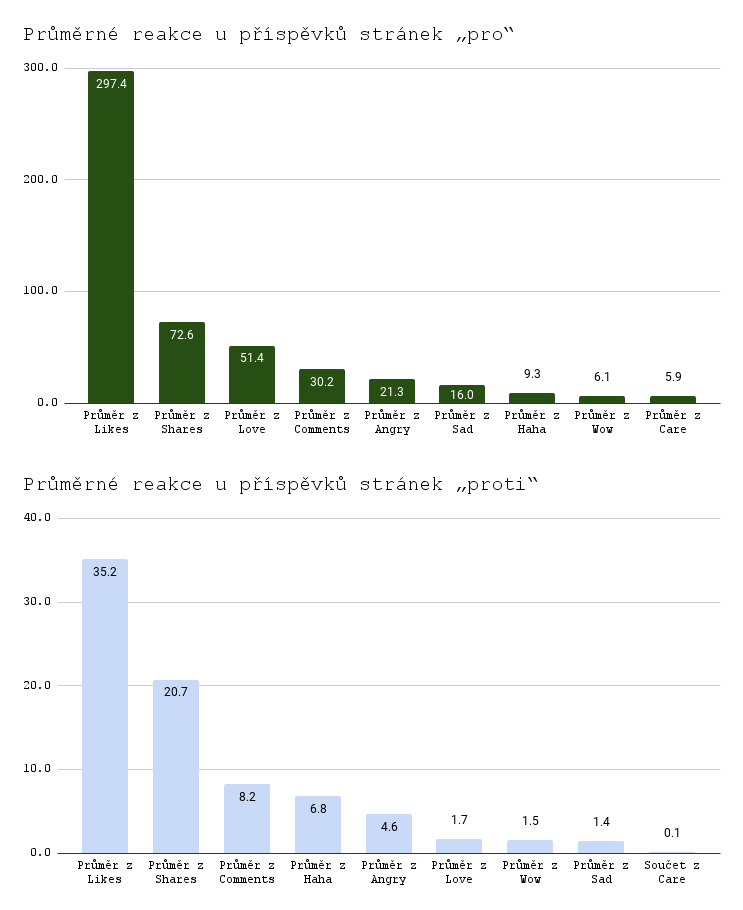
\includegraphics[width=14cm]{obrazky/Průměrné reakce u příspěvků stránek.png}
        \centering
        \caption[Průměrné interakce na stránkách \uv{pro} a \uv{proti}]{Průměrné interakce na stránkách \uv{pro} a \uv{proti} od nejvíce používaných po nejméně používané. Zdroj: vlastní zpracování}
        \label{fig:fb-klima-stranky-reakce}
    \end{figure}